% CS6140 Homework Assignment Template
% Computer Science
% Northeastern University
% Boston, MA 02115

% Do not manipulate any of the settings
\documentclass[twoside]{article}

\usepackage{epsfig}
\usepackage{natbib}
\usepackage{units}
\usepackage{amssymb}
\usepackage{amsmath}
\usepackage{babel}
\usepackage{graphicx}
\graphicspath{ {./images/} }

\setlength{\oddsidemargin}{0 in}
\setlength{\evensidemargin}{0 in}
\setlength{\topmargin}{-0.6 in}
\setlength{\textwidth}{6.5 in}
\setlength{\textheight}{8.5 in}
\setlength{\headsep}{0.75 in}
\setlength{\parindent}{0 in}
\setlength{\parskip}{0.1 in}

\newcommand{\lecture}[3]{
   \pagestyle{myheadings}
   \thispagestyle{plain}
   \newpage
   \setcounter{page}{1}
   \noindent
   \begin{center}
   \framebox{
      \vbox{\vspace{2mm}
    \hbox to 6.28in { {\bf CS6140: Machine Learning\hfill} }
       \vspace{6mm}
       \hbox to 6.28in { {\Large \hfill #1  \hfill} }
       \vspace{6mm}
       \hbox to 6.28in { {\it Assigned: #2 \hfill Due: #3} }
      \vspace{2mm}}
   }
   \end{center}
   \markboth{#1}{#1}
   \vspace*{4mm}
}

\begin{document}

% to have alphanumeric enumeration (Hasan's command)
\renewcommand{\labelenumi}{\alph{enumi})}

\lecture{Homework Assignment \# 1}{01/21/2020}{02/04/2020, 11:59pm, through Blackboard}
\textbf{Seyed Ali Sadat Akhavani}

\textbf{sadatakhavani.s@husky.neu.edu}

---

\begin{center}
Eight questions, 135 points in total. Good luck!\\
Prof. Predrag Radivojac, Northeastern University
\end{center}

%%
%% Problem
%%

\textbf{Problem 1.} (5 points) Let $(\Omega, \mathcal{A}, P)$ be a probability space and $A \subseteq \Omega$ and $B \subseteq \Omega$ any two subsets of $\Omega$. Prove the following expression or provide a counterexample if it does not hold
\[
P(A) = P(A|B) + P(A | B^c),
\]
\noindent where $A^c$ is the complement of $A$.



\textbf{Solution:}
\newline
This is wrong. Consider that A and B are mutually exclusive. So $(A \cap B = 0)$ and $(A \cap B^c = A)$
\[
P(A|B) + P(A | B^c) = \frac{P(A \cap B)}{P(B)} + \frac{P(A \cap B^c)}{P(B^c)} = \frac{0}{P(B)} + \frac{P(A \cap B^c)}{P(B^c)} = \frac{P(A)}{P(B^c)} \neq P(A)
\]

%%
%% Problem
%%

\textbf{Problem 2.} (15 points) Let $X$ be a random variable on $\mathcal{X}=\left\{ a,b,c\right\}$ with the probability mass function $p(x)$. Let $p(a)=0.1$, $p(b)=0.2$, and $p(c)=0.7$ and some function $f(x)$ be 
\[
f(x)=\begin{cases}
10 & x=a\\
5 & x=b\\
\frac{10}{7} & x=c
\end{cases}
\]
\begin{enumerate}
\item (5 points) What is $\mathbb{E}[f(X)]$?


\textbf{Solution:}
\[
\mathbb{E}[f(X)] = \Sigma_{x\in \chi}^{}{f(x)p(x)} = f(a)p(a) + f(b)p(b) + f(c)p(c) = 10 * 0.1 + 5 * 0.2 + \frac{10}{7} * 0.7 = 1 + 1 + 1 = 3
\]


\item (5 points) What is $\mathbb{E}[1/p(X)]$?


\textbf{Solution:}
\[
\mathbb{E}[1/p(X)] = \Sigma_{x\in \chi}^{}{\frac{1}{p(x)}.p(x)} = \Sigma_{x\in \chi}^{}{1} = 1 + 1 + 1 = 3
\]



\item (5 points) For an arbitrary finite set $\mathcal{X}$ with $n$ elements and arbitrary $p(x)$ on $\mathcal{X}$, what is $\mathbb{E}[1/p(X)]$?


\textbf{Solution:}
As we saw in the previous part, the product of $\frac{1}{p(x)} . p(x) = 1$ so the result of $\mathbb{E}[1/p(X)]$ only depends on the length of $\chi$ which is n. So $\mathbb{E}[1/p(X)] = n$

\end{enumerate}

%%
%% Problem
%%

\textbf{Problem 3.} (10 points) Let $X$ and $Y$ be random variables. Prove or disprove the following formula
\[
V[X+Y]=V[X]+V[Y]+2\textrm{Cov}[X,Y],
\]
where $V[X]$ is the variance of $X$ and $\textrm{Cov}[X,Y]$ is the covariance between $X$ and $Y$.


\textbf{Solution:}
\[
V[X+Y] = ( (x+y) - \mathbb{E}[X+Y])^2 = (x+y - \mathbb{E}[X] - \mathbb{E}[Y])^2 = ( (x - \mathbb{E}[X]) + (y - \mathbb{E}[Y]) )^2 = 
\]
\[
(x-\mathbb{E}[X])^2 + (y-\mathbb{E}[Y])^2 + 2(x-\mathbb{E}[X])(y-\mathbb{E}[Y]) = V[X] + V[Y] + 2\textrm{Cov}[X,Y]
\]


%%
%% Problem
%%

\textbf{Problem 4.} (20 points) Suppose that the number of accidents occurring daily in a certain plant has a Poisson distribution with an unknown mean $\lambda$. Based on previous experience in similar industrial plants, suppose that our initial feelings about the possible value of $\lambda$ can be expressed by an exponential distribution with parameter $\theta = \frac{1}{2}$ is, the prior density is
\[
p(\lambda) = \theta e ^ {-\theta \lambda}
\]
where $\lambda \in (0, \infty)$. If there are 99 accidents over the next 11 days, determine
\begin{enumerate}
\item (5 points) the maximum likelihood estimate of $\lambda$

\textbf{Solution:}
\[
f_{ML} = arg\max_{\lambda \in (0, \infty)} {p(D|f)} = \Pi_{i=1}^{n}{p(x_i | \lambda) = \frac{\lambda^{\Sigma_{i=1}^{n}{x_i}} . e^{-n\lambda}}{\Pi_{i=1}^{n}{x_i!}}}
\]
\[
ll(D,\lambda) = \ln\lambda\Sigma_{i=1}^{n}{x_i} - n\lambda - \Sigma_{i=1}^{n}{\ln(x_i!)}
\]
\[
\frac{\partial ll(D,\lambda)}{\partial \lambda} = \frac{1}{\lambda} \Sigma_{i=1}^{n}{x_i} - n = 0
\]
\[
\lambda_{ML} = \frac{1}{n} \Sigma_{i=1}^{n}{x_i} = \frac{99}{11} = 9
\]

\item (5 points) the maximum a posteriori estimate of $\lambda$

\textbf{Solution:}
\[
f_{ML} = arg\max_{\lambda \in (0, \infty)} {p(D|f)p(f)}
\]
We know that:
\[
p(D | \lambda) = \frac{\lambda^{\Sigma_{i=1}^{n}{x_i}} . e^{-n\lambda}}{\Pi_{i=1}^{n}{x_i!}}
\]
We maximize ln of the posterior distribution $p(\lambda | D)$
\[
\ln p(\lambda | D) = \ln p(D|\lambda) + \ln p(\lambda)
= ll(D,\lambda) = \ln\lambda\Sigma_{i=1}^{n}{x_i} - n\lambda - \Sigma_{i=1}^{n}{\ln(x_i!)} + \ln \theta - \theta \lambda
\]
Now we will make the derivative of this result to zero in order to find the $\lambda_{MAP}$
\[
\frac{1}{\lambda} \Sigma_{i=1}^{n}{x_i} - n - \theta = 0
\]
\[
\lambda_{MAP} = \frac{\Sigma_{i=1}^{n}{x_i}}{n+\theta} = \frac{99}{11 + 0.5} = 8.6
\]

\item (10 points) the Bayes estimate of $\lambda$.

\textbf{Solution:}
We want to find $\mathbb{E}[\Lambda | D]$ first we should write this:
\[
p(\lambda|D) = \frac{p(D|\lambda)p(\lambda}{\int_0^\infty p(D|\lambda)p(\lambda)d\lambda}
\]
We have that:
\[
p(D|\lambda) = \frac{\lambda^{\Sigma_{i=1}^{n}{x_i}} . e^{-n\lambda}}{\Pi_{i=1}^{n}{x_i!}}
\]
we also have:
\[
p(\lambda) = \theta e^{-\theta \lambda}
\]
So now we should calculate:
\[
p(D) = \int_0^\infty{p(D|\lambda)p(\lambda)d\lambda} = \int_0^\infty{{\frac{\lambda^{\Sigma_{i=1}^{n}{x_i}} . e^{-n\lambda}}{\Pi_{i=1}^{n}{x_i!}}}.{\theta e^{-\theta \lambda}}d\lambda} =
\frac{\theta}{\Pi_{i=1}^n{x_i!}} \int_0^\infty{\lambda^{\Sigma_1^n{x_i}}.e^{-(n+\theta)\lambda}d\lambda}
\]
We can simplify this integral based on some know rules. The result will be:
\[
p(D) = \frac{\theta}{\Pi_{i=1}^n{x_i!}} .
\frac{\Gamma(\Sigma_1^n{x_i + 1})}{(n+\theta)^{\Sigma_1^n{x_i + 1}}}
\]
Now we will calculate $p(\lambda|D)$
\[
p(\lambda|D) = 
\frac{p(D|\lambda)p(\lambda)}{p(D)} =
{\frac{\lambda^{\Sigma_{i=1}^{n}{x_i}} . e^{-n\lambda}}{\Pi_{i=1}^{n}{x_i!}}}.{\theta e^{-\theta \lambda}} . 
\frac{\Pi_{i=1}^n{x_i!}}{\theta} .
\frac{(n+\theta)^{\Sigma_1^n{x_i + 1}}}{\Gamma(\Sigma_1^n{x_i + 1})} =
\frac{\lambda^{\Sigma_1^n{x_i}} . (n+\theta)^{\Sigma_1^n{x_i + 1}} . e^{-\lambda(n+\theta)} } {\Gamma(\Sigma_1^n{x_i} + 1)}
\]
Finally, we have:
\[
\mathbb{E}[A|D] = \int_0^\infty{\lambda p(\lambda|D)d\lambda} = 
\frac{(n+\theta)^{\Sigma_1^n{x_i} + 1})}{\Gamma(\Sigma_1^n{x_i}+1)} .
\int_0^\infty{\lambda^{\Sigma_1^n{x_i}+1} . e^{-\lambda(n+\theta)} d\lambda} =
\frac{\Gamma(\Sigma_1^n{x_i} + 2)}{\Gamma(\Sigma_1^n{x_i}+1).(n+\theta)} =
\]
\[
\frac{\Sigma_1^n{x_i}+1}{n+\theta} = \frac{99+1}{11+0.5} = 8.69
\]

\end{enumerate}

%%
%% Problem
%%

\textbf{Problem 5.} (10 points) Let $\mathcal{D}=\left\{ x_i\right\}_{i=1}^n$ be an i.i.d.~sample from
\[
p(x)=\begin{cases}
e^{-(x-\theta_0)} & x \geq \theta_0\\
0 & \textrm{otherwise}
\end{cases}
\]
\noindent Determine $\theta_{\textrm{ML}}$ -- the maximum likelihood estimate of $\theta_0$. 

\textbf{Solution:}

The likelihood function is:
\[
p(D|\theta) = \Pi_{i=1}^n{p(x_i|\theta)} = 
\begin{cases}
e^{n \theta_0 - \Sigma_{i=1}^n{x_i}} & x_i \geq \theta_0\\
0 & \textrm{otherwise}
\end{cases}
\]
We know that $e^{n \theta_0 - \Sigma_{i=1}^n{x_i}}$ is an increasing function of $\theta$ so the biggest possible value of $\theta$ such that $x_i \geq \theta_0$ for $i=1,...,n$ is: $\theta = \min(x_1,...,x_n)$ 
So Maximum Likelihood of $\theta$ is $\theta_0 = \min(x_1,...,x_n)$


%%
%% Problem
%%

\textbf{Problem 6.} (25 points) Let $\mathcal{D}=\left\{ x_{i}\right\} _{i=1}^{n}$, where $x_i \in \mathbb{R}$, be a data set drawn independently from a Gumbel distribution
\[
p(x)=\frac{1}{\beta}e^{-\frac{x-\alpha}{\beta}}e^{-e^{-\frac{x-\alpha}{\beta}}},
\]
where $\alpha\in\mathbb{R}$ is the location parameter and $\beta>0$ is the scale parameter. 
\begin{enumerate}
\item (10 points) Derive an algorithm for estimating $\alpha$ and $\beta$.

\textbf{Solution:}

We will use Maximum Likelihood to solve this.
\[
p(D|\alpha, \beta) = \Pi_{i=1}^{n}{\frac{1}{\beta}e^{-\frac{x_i-\alpha}{\beta}}e^{-e^{-\frac{x_i-\alpha}{\beta}}}}
\]
The log-likelihood function would be:
\[
ll(D|\alpha, \beta) = -n ln\beta - \Sigma_1^n{\frac{x_i - \alpha}{\beta}} - \Sigma_1^n{e^{-\frac{x_i - \alpha}{\beta}}}
\]
The $\alpha$ derivative is:
\[
\frac{\partial}{\partial \alpha} ll(D|\alpha, \beta) = 
\frac{n}{\beta} - \frac{\Sigma_1^n{e^{-\frac{x_i - \alpha}{\beta}}}}{\beta}
\]
We see that $\beta$ is also in $\alpha$ derivative.

The $\beta$ derivative is:
\[
\frac{\partial}{\partial \beta} ll(D|\beta, \beta) = 
\frac{n}{\beta} - \Sigma_1^n{\frac{x_i - \alpha}{\beta^2}} - \Sigma_1^n{\frac{x_i - \alpha}{\beta^2} . e^{-\frac{x_i - \alpha}{\beta}}}
\]
We see that $\alpha$ is also in $\beta$ derivative.
So we need to use gradient descent in order to estimate $\alpha$ and $\beta$ which we will use it in the next part of the question. We have to guess a value for $\alpha$ and $\beta$ and then use gradient descent to make our guess better and achieve the best possible result. I will talk about step size, learning rate and other stuff in part c. More information is also visible in the code


\item (10 points) Implement the algorithm derived above and evaluate it on data sets of different sizes. First, find or develop a random number generator that creates a data set with $n \in \left\{ 100, 1000, 10000 \right\}$ values using some fixed $\alpha$ and $\beta$. Then make at least 10 data sets for each $n$ and estimate the parameters. For each $n$, report the mean and standard deviation on the estimated $\alpha$ and $\beta$. If $n=10000$ is too large for your computing resources, skip it.

\textbf{Solution:}

When n=100:

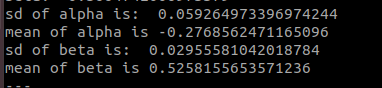
\includegraphics[]{images/n100.png}


When n=1000

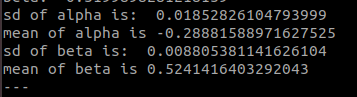
\includegraphics[]{images/n1000.png}

If you need more information, you can see the code and run it.


\item (5 points) The problem above will require you to implement an iterative estimation procedure. You will need to decide on how to initialize the parameters, how to terminate the estimation process and what the maximum number of iterations should be. Usually, some experimentation will be necessary \emph{before} you run the experiments in part (b) above. Summarize what you did in a short paragraph, no more than two paragraphs.

\textbf{Solution:}

We are using gradient descent to solve this problem.
In this method we have to choose learning rate, number of iterations, and an initial estimation for $\alpha$ and $\beta$. For alpha and beta, I chose value $\alpha=0$ and $\beta=1$ randomly which ended well and the results that I received where not too far from these valuse. I also tried different values but these estimations were good enough.
For the learning rate and number of iterations, I started with iterations=100 and learning-rate=0.01 but after running the code I realized that I am not getting good results because likelihood was not increasing well. So I tried to increase number of iterations and also decreasing the learning rate in order to achieve better results. I stopped the algorithm (iterations) when I didn't see any more increase to the likelihood and this means we have reached the local maximum.

\end{enumerate}
NB: There are several versions and naming conventions for the Gumbel distribution in the literature.

%%
%% Problem
%%

\textbf{Problem 7.} (30 points)  Let $\mathcal{D}=\left\{ x_{i}\right\} _{i=1}^{n}$, where $x_i \in \mathbb{R}$, be a data set drawn independently from the mixture of two distributions
\[
p(x)=w_{1}p_{1}(x)+w_{2}p_{2}(x),
\]
where 
\[
p_{1}(x)=\frac{1}{\beta}e^{-\frac{x-\alpha}{\beta}}e^{-e^{-\frac{x-\alpha}{\beta}}},
\]
is a Gumbel distribution with parameters $\alpha$ and $\beta$, 
\[
p_{2}(x)=\frac{1}{\sqrt{2\pi\sigma^{2}}}e^{-\frac{(x-\mu)^{2}}{2\sigma^{2}}},
\]
is a Gaussian distribution with parameters $\mu$ and $\sigma$, and $(w_{1},w_{2})$ are positive constants such that $w_{1}+w_{2}=1$.
\begin{enumerate}
\item (15 points) Derive an EM algorithm for estimating $w_1$, $w_2$, $\alpha$, $\beta$, $\mu$ and $\sigma$.

\textbf{Solution:}

E-Step: Compute $p(y|D, \theta^{(t)})$

M-Step: Compute $\theta^{(t+1)}$


The steps would be like this:
1- Initialize $\alpha^0, \beta^0, \sigma^0, \mu^0$ and $w1^0 and w2^0$
2- t=0
loop:
\[
w_k^{(t+1)} = \frac{1}{n} \Sigma_1^n{p_{Y_i}(k|x_i, \theta^{(t)})}
\]
we should write this for all four parameters ($\alpha, \beta, \sigma, \mu$)
\[
\alpha_k^{(t+1)} = \frac{ \Sigma_1^n{p_{Y_i}(k|x_i, \theta^{(t)}) } }
{\Sigma_1^n{x_i p_{Y_I} (k|x_i, \theta^{(t)}) }}
\]
the below expression should be written for all parameters too:
\[
p_{Y_i}(k|x_i, \theta^{(t)}) = \frac{w_k^{(t)} p(x_i|\alpha_k^{(t)})}
{\Sigma_{j=1}^m{w_j^{(t)} p(x_i|\alpha_j^{(t)} })}
\]
\[t=t+1\]

These are the steps and functions. They are computed in the code.

\item (15 points) Implement the algorithm derived above and evaluate it on data sets of different sizes. Use similar experimentation as in Problem 3.

\textbf{Solution:}

I have written the code but it is not complete. The main idea is implemented but it still needs work.
\end{enumerate}
You can recycle derivations and code from Problem 6. You can also use any result and derivation from the lecture notes posted on the class web site.

%%
%% Problem
%%
\textbf{Problem 8.} (20 points) Understanding the curse of dimensionality. Consider the following experiment: generate $n$ data points with dimensionality $k$. Let each data point be generated using a uniform random number generator with values between $0$ and $1$. Now, for a given $k$, calculate
\[
r(k)=\log_{10}\frac{d_{\max}(k)-d_{\min}(k)}{d_{\min}(k)}
\]
\noindent where $d_{\max}(k)$ is the maximum distance between any pair of points and $d_{\min}(k)$ is minimum distance between any pair of points (you cannot use identical points to obtain the minimum distance of 0). Let $k$ take each value from $\left\{ 1,2,\ldots,99,100\right\}$. Repeat each experiment multiple times to get stable values by averaging the quantities over multiple runs for each $k$. 

\begin{enumerate}
\item (15 points) Plot $r(k)$ as a function of $k$ for two different values of $n$; $n \in \left\{ 100, 1000 \right\}$. Label and scale each axis properly to be able to make comparisons over different $n$'s. Embed your final picture(s) in the file you are submitting for this assignment.

\textbf{Solution:}

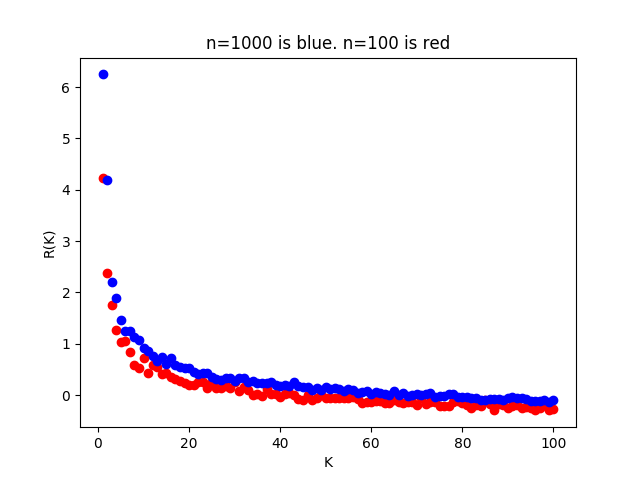
\includegraphics[]{q8.png}

\item (5 points) Discuss your observations and also compare the results to your expectations before you carried out the experiment.

\textbf{Solution:}

As we see in the picture above, 
We want to show that as the number of dimensions grows, the amount of data we need to generalise accurately grows exponentially. This can be seen in the picture obviously, as expected. We also see that when we increase the "n=1000", the output of the function is always better than n=100. This is completely in line with what we though. We need to give more data as the dimensionality grows. We see that the blue dots (n=1000) are always above red dots (n=100) and total value of the function decreases when k increases.



\end{enumerate}


% \input{policies.tex}

\end{document}

